\subsection{Configuration Management Plan}
This software project consists of 5 official documents including SRS, SPMP, SDD, Testing report and User Manuel), meeting agenda and minutes, and software for operating EV3 robot. All these configuration items’ standards are developed by documentation manager and monitored by quality manager. All team members are responsible for following this configuration standard during the whole project life cycle. The detail software and testing components will be mentioned in SDD document and testing report.
GitHub Repository structure
The repository structure is built based on the component of the project. The highest level of repository is Code and Documentation. The below is the detail GitHub Repository structure:

\subsection{GitHub Repository structure}
The repository structure is built based on the component of the project. The highest level of repository is Code and Documentation. the detail GitHub Repository structure is shown on fig.3.

\begin{figure}[H]
	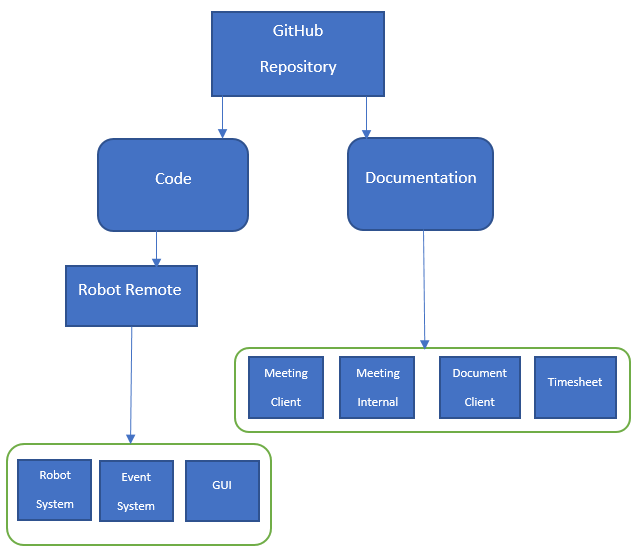
\includegraphics[width=\linewidth]{GIT.png}  % created using www.draw.io
	\caption{GITHUB repository}
	\label{fig:GITHUB repository}				
\end{figure}

\subsection{Configuration Naming System and version control}
Any draft of configuration items shall be followed as below naming standards:
\begin{itemize}
\item \texttt{\detokenize{<Title>_<version>.<extension>}}\\
      \texttt{\detokenize{For examples: SRS_v0.9.tex}}
\item The Final version is v1.0. The draft version will be named as v0.1-v0.9.
\item The modified date for each sub-version shall be mentioned in revision history table which is included into documents.\\
\end{itemize}

The examples of revision history for SRS-v0.9.tex is shown on Table2 :\\

\begin{table}[]
	\centering
	\caption{Revision history}
	\label{my-label}
	\begin{tabular}{|l|l|l|l|}
		\hline
		Name      & Date      & Version & Summary of Changes           \\ \hline
		1st Draft & 21/8/2017 & 0.9.1   & Initial Draft                \\ \hline
		2nd Draft & 22/8/2017 & 0.9.2   & Identification numbers added \\ \hline
	\end{tabular}
\end{table}


The revision table for final version shall include all the change for each version. After final version released, any change is required a change request which is mentioned in section 8.3.\\


The meeting agenda and meeting minutes shall follow as below naming system:\\
\texttt{\detokenize{<Title>_<Type>_<week>.<extension>}}\\
\begin{itemize}
\item Title: Agenda or Minutes
\item Type: Client or Internal
\end{itemize}
\texttt{\detokenize{For example: agenda_client_week3.tex, minutes_internal_week3.tex}} \\\\
Usually, there are only one client meeting and internal group meeting per week. If there are any emergency meeting, the date should be included.\\\\
\texttt{\detokenize{For example: agenda_internal_week3_17082017.tex}}\\
\texttt{\detokenize{The date format shall be <days><months><year>}}\\
\subsection{Change request handling}
There are two types change request handling. Documentation and Software change request handling.\\
Documentation:\\\\
The Documents will be divided by documentation manager into difference sub-tasks for each team member to edit their own parts. Team members can make any change on their own part before the final version release. Team members is required to edit the revision table to record their change on the document. The documentation review meeting will be held by documentation manager to review all the changes on the document before releasing final version. After the review meeting, documentation manager will decide whether the quality of the document is accepted. If the quality is acceptable, the final version of the document will be released and no change is allowed. If the quality is unacceptable, documentation manager need to determine another deadline for the change of document and assign duties to each team member. Another review meeting is required for releasing final version document.
If team member has a strong reason to change the final version document, documentation manager must need to establish a review meeting to discuss this change.\\\\
Software:\\
Team member must need to create new branch in github repository to make a change or add new function on software. The change on this branch must not affect master branch. Regular software review meeting will be held by development manager to review all the team member’s work and discuss the potential issue for merging the work to master branch. \\\\